\subsection{Zeeman splitting of $^{87} {\rm Rb}$ hyperfine ground states}\label{zeeman chpt}
The angular momentum of $^{87} {\rm Rb}$ interacts with the external magnetic field and the hyperfine states split into sub-states. Here we use perturbation theory to calculate the energy of each sub-states of $^{87} {\rm Rb}$ ground state.

For the $^{87} {\rm Rb}$ ground state, $J=1/2$ and $I=3/2$. It has hyperfine states $\ket{F=1}$ and $\ket{F=2}$. The Hamiltonian with external magnetic field is 
\begin{equation}
    \hat{H} = \hat{H}_{hfs} + (\mu_B g_J\Vec{J} + \mu_N g_I\Vec{I})\Vec{B}.
\end{equation}
Here $\mu_B = 9.27\times 10^{-24} {\rm J}\cdot {\rm T}^{-1}$ is Bohr magneton, the natural unit for expressing the magnetic moment of an electron caused by either its orbital or spin angular momentum. $\mu_N = 5.05\times 10^{-27} {\rm J}\cdot {\rm T}^{-1}$ is the nuclear magneton. $g_J$ and $g_I$ are land\'e g-factors. For $^{87} {\rm Rb}$ ground state, $g_J \approx 2.00233$ and $g_I \approx -0.00099$. 

Define the direction of magnetic field z, the Hamiltonian can be represented by the z-component of angular momentum
\begin{equation}
    \hat{H} = \hat{H}_{hfs} + \mu_B(g_J m_J + g_Im_I)B,
\end{equation}
where $m_J$ and $m_I$ are magnetic quantum numbers. $\hat{H}_{hfs}$ is diagonal in the basis of $\{\ket{F,m_F}\}$, and we can proceed by representing states $\ket{J=1/2,m_J,I=3/2,m_I}$ with $\{\ket{F,m_F}\}$ and calculate the energy of states $\ket{F,m_F}$ to second order.

\begin{align}
    &\ket{\frac{1}{2},\frac{3}{2}} = \ket{2,2}, &&\ket{\frac{1}{2},\frac{1}{2}} = \frac{\sqrt{3}}{2}\ket{2,1} - \frac{1}{2}\ket{1,1}\\\nonumber
    &\ket{\frac{-1}{2},\frac{3}{2}} = \frac{1}{2}\ket{2,1} + \frac{\sqrt{3}}{2}\ket{1,1}, &&\ket{\frac{-1}{2},\frac{1}{2}} = \frac{1}{\sqrt{2}}\ket{2,0} + \frac{1}{\sqrt{2}}\ket{1,0}\\ \nonumber
    &\ket{\frac{1}{2},\frac{-1}{2}} = \frac{1}{\sqrt{2}}\ket{2,0} - \frac{1}{\sqrt{2}}\ket{1,0}, &&\ket{\frac{1}{2},\frac{-3}{2}} = \frac{1}{2}\ket{2,-1} - \frac{\sqrt{3}}{2}\ket{1,-1}\\ \nonumber
    &\ket{\frac{-1}{2},\frac{-1}{2}} = \frac{\sqrt{3}}{2}\ket{2,-1} - \frac{1}{2}\ket{1,-1}, &&\ket{\frac{-1}{2},\frac{-3}{2}} = \ket{2,-2}\\ \nonumber
\end{align}

In the $\{\ket{F,m_F}\}$ basis,
\begin{equation}
    \hat{H}_{hfs}\ket{F,m_F} = E_{F}\ket{F,m_F}.
\end{equation}
Treat the interaction with the external magnetic field as a perturbation, the first-order perturbed energy for state $\ket{F,m_F}$ is
\begin{equation}
    \Delta E_1 = \matrixel{F,m_F}{(g_J\Vec{J}_z + g_I\Vec{I}_z)}{F,m_F}\mu_B B,
\end{equation}
and the second order perturbed energy is
\begin{equation}
    \Delta E_2 = \sum_{F',m_F'} \frac{|\matrixel{F,m_F}{(g_J\Vec{J}_z + g_I\Vec{I}_z)}{F',m_F'}|^2}{E_F-E_{F'}}(\mu_B B)^2.
\end{equation}

The energy of $\ket{F,m_F}$ states are listed here, in the units of ${\rm MHz}$, ${\rm MHz/G}$ and ${\rm MHz/G^2}$. The numbers are useful for quick estimation of the magnetic field in the lab.
\begin{align}
    \ket{2,2} &= 2.75\times 10^3h ~{\rm MHz} + 1.405h~{\rm MHz/G}\times B + 0h ~{\rm MHz/G^2}\times B^2\\\nonumber
    \ket{2,1} &= 2.75\times 10^3h ~{\rm MHz} + 0.7026h~{\rm MHz/G}\times B + 2.879\times 10^{-4}h ~{\rm MHz/G^2}\times B^2\\\nonumber
    \ket{2,0} &= 2.75\times 10^3h ~{\rm MHz} + 0h~{\rm MHz/G}\times B + 3.839\times 10^{-4}h ~{\rm MHz/G^2}\times B^2\\\nonumber
    \ket{2,-1} &= 2.75\times 10^3h ~{\rm MHz} - 0.7026h~{\rm MHz/G}\times B + 2.879\times 10^{-4}h ~{\rm MHz/G^2}\times B^2\\\nonumber
    \ket{2,-2} &= 2.75\times 10^3h ~{\rm MHz} - 1.405h~{\rm MHz/G}\times B + 0h ~{\rm MHz/G^2}\times B^2\\\nonumber
    \ket{1,1} &= -4.2896\times 10^3h ~{\rm MHz} - 0.7052h~{\rm MHz/G}\times B - 2.879\times 10^{-4}h ~{\rm MHz/G^2}\times B^2\\\nonumber
    \ket{1,0} &= -4.2896\times 10^3h ~{\rm MHz} + 0h~{\rm MHz/G}\times B - 2.879\times 10^{-4}h ~{\rm MHz/G^2}\times B^2\\\nonumber
    \ket{1,-1} &= -4.2896\times 10^3h ~{\rm MHz} + 0.7052h~{\rm MHz/G}\times B - 2.879\times 10^{-4}h ~{\rm MHz/G^2}\times B^2\\\nonumber
\end{align}

The second-order perturbation leads to the quadratic Zeeman shift which has a sizable effect when the magnetic field on the order of $ 10{\rm G}$. In some our experiments, the quadratic Zeeman shift makes the energy difference between $\ket{1,0}$ and $\ket{1,-1}$ large enough than the difference between $\ket{1,0}$ and $\ket{1,1}$. So we can effectively treat the $F=1$ manifold as a two-level system by decoupling $\ket{1,-1}$. 

For larger magnetic field, larger than $10^3{\rm G}$, the perturbation theory breaks down and {\bf Breit-Rabi formula} \cite{breit1931measurement} is useful in the case $J=1/2$. 
\begin{align}
     &E_{F=I\pm1/2} = -\frac{A_{hfs}}{4} + m_Fg_I\mu_NB \pm A_{hfs}\sqrt{1 + m_Fx x^2}, m_F \neq 2, -2\\ \nonumber
     &E_{F=2,m_F=\pm2} = -\frac{A_{hfs}}{4} + m_Fg_I\mu_NB + A_{hfs}(1 \pm x) \\\nonumber
     &x = \frac{(g_J\mu_B - g_I\mu_N)B}{2A_{hfs}}\\\nonumber
\end{align}
The energy of states $\ket{F,m_F}$ is shown in Fig.~(\ref{fig:BField}) for the magnetic field up to 15000 {\rm G}.

\begin{figure}[htbp]
    \centering
    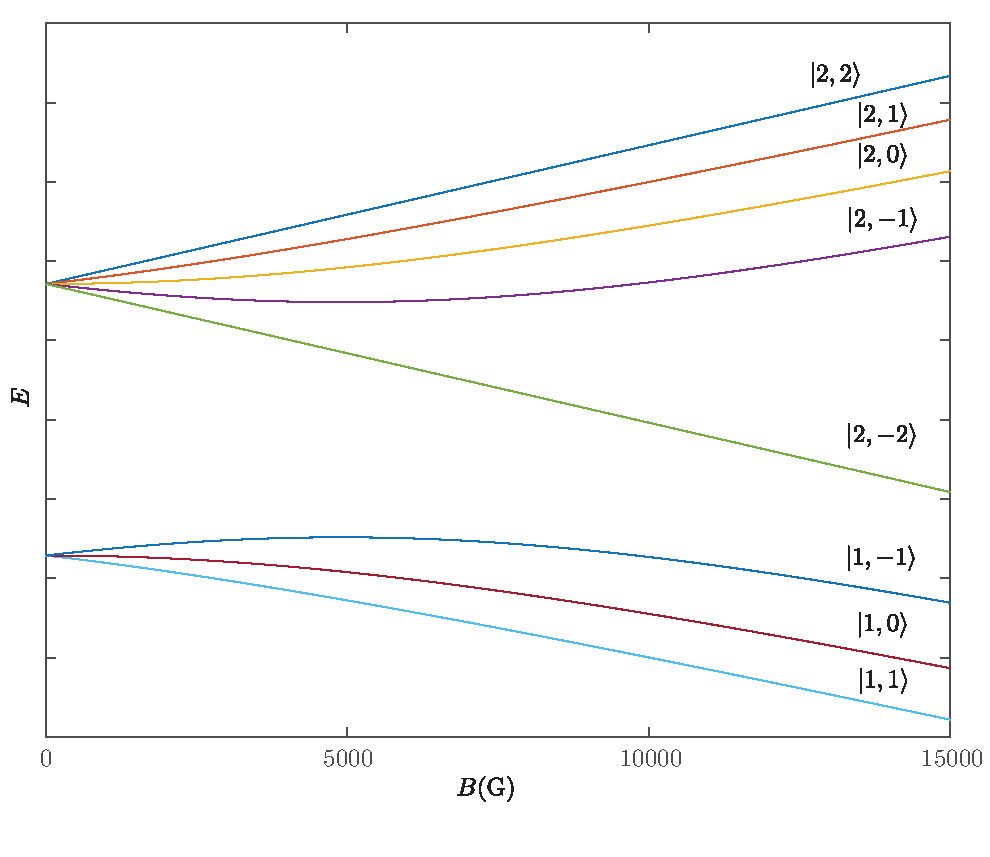
\includegraphics[width=\textwidth]{Chapter2_secs/B_field.pdf}
    \caption{Zeeman splitting of $^{87} {\rm Rb}$ ground states $\ket{F,m_F}$. }
    \label{fig:BField}
\end{figure}